\documentclass[tikz,border=10pt]{standalone}
\usetikzlibrary{calc}
\begin{document}
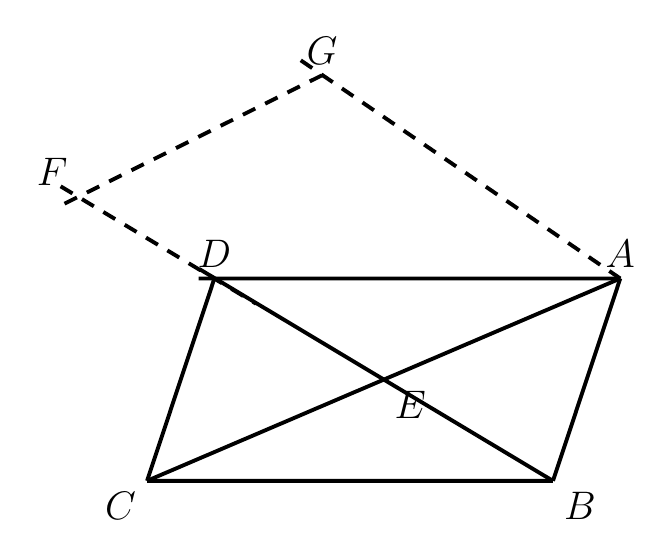
\begin{tikzpicture}[line width=1.4pt, line join=round,
  lbl/.style={font=\fontsize{15}{18}\selectfont}]
  % Vertices (pixel -> cm, s=0.01214, cx=404, cy=325)
  \coordinate (A) at (3.437812352877226,-0.050524953273600126);
  \coordinate (B) at (2.582736673407033,-2.6209079387586987);
  \coordinate (C) at (-2.5722056343088964,-2.6205095825524634);
  \coordinate (D) at (-1.7173744877199921,-0.05086167019895793);
  \coordinate (E) at (0.4289373879098429,-1.337170422201492);
  \coordinate (F) at (-3.439893117832552,0.9899308666178529);
  \coordinate (G) at (-0.35001317433266194,2.5300437003673584);
  % Segment end points from GES
  \coordinate (DAleft) at (-1.917374487719992,-0.05086167019895793);   % D-A line start
  \coordinate (BDend) at (-1.907374487719992,0.06913832980104208);     % B-D line end past D
  \coordinate (GAext) at (-0.620013174332662,2.7200437003673588);     % dashed G-A beyond G
  \coordinate (FGext) at (-3.619893117832552,0.8999308666178529);     % dashed F-G beyond F
  \coordinate (FDstart) at (-3.669893117832552,1.1199308666178531);   % dashed F-D beyond F
  \coordinate (FDend) at (-1.187374487719992,-0.37086167019895794);    % dashed F-D beyond D

  % Solid edges
  \draw[line join=round] (A) -- (C);
  \draw[line join=round] (DAleft) -- (A);
  \draw[line join=round] (C) -- (B);
  \draw[line join=round] (BDend) -- (B);
  \draw[line join=round] (D) -- (C);
  \draw[line join=round] (A) -- (B);

  % Dashed auxiliary lines
  \draw[dashed, dash pattern=on 5pt off 4pt, line join=round] (GAext) -- (A);
  \draw[dashed, dash pattern=on 5pt off 4pt, line join=round] (FGext) -- (G);
  \draw[dashed, dash pattern=on 5pt off 4pt, line join=round] (FDstart) -- (FDend);

  % Vertex labels (outside the figure)
  \node[above, lbl] at (A) {$A$};
  \node[below right, lbl] at (B) {$B$};
  \node[below left, lbl] at (C) {$C$};
  \node[above, lbl] at (D) {$D$};
  \node[below right, lbl] at (E) {$E$};
  \node[above left, lbl] at (F) {$F$};
  \node[above, lbl] at (G) {$G$};
\end{tikzpicture}
\end{document}
% GEOAGENT_REPAIR_V1 c18a466396f54661 dfd2b5e41ef378e7681dde274a804ee943a5519877d26c194480b51d63416b60